\section{Alberi binari di ricerca}
Gli alberi binari di ricerca sono alberi in cui per ogni nodo $n$: 
\begin{enumerate}
    \item Il valore di ogni chiave contenuta nel sottoalbero sinistro di $n$ è minore o uguale alla chiave di $n$
    \item Il valore di ogni chiave contenuta nel sottoalbero destro di $n$ è maggiore della chiave di $n$
\end{enumerate}
Una visita in ordine simmetrico di un A.B.R. produce un elenco ordinato per chiave.\\
Se devo trovare il nodo con chiave massima scendo tutto a destra, per quello di chiave minima tutto a sinistra.\\
Il costo di inserimento, ricerca e cancellazione è $O(altezza)$.
Il massimo numero di nodi di un albero di altezza $h$ è $2^{h+1}-1$, quindi:
\begin{itemize}
    \item $h + 1 \le n \le 2^{h+1}-1$
    \item $\log_2(n+1) - 1 \le h \le n - 1$
\end{itemize}
Vogliamo fare in modo che l'albero rimanga più bilanciato possibile in modo
da evitare il caso peggiore.

\subsection{Operazioni}
Vediamo ora l'implementazione di alcune operazioni eseguibili sugli alberi binari di ricerca.
\begin{algorithm}
    \caption{Ricerca del massimo}
    \Indm\textbf{Funzione} \emph{massimo (AlberoRicerca r)} $\rightarrow Nodo$\\
    \Indp\eIf{$r = null$}{\Return $null$}{
        $n \leftarrow r$\\
        \While{$n.dx \neq null$}{
            $n \leftarrow n.dx$
        }
        \Return{$n$}
    }
\end{algorithm}

\begin{algorithm}
    \caption{Ricerca del minimo}
    \Indm\textbf{Funzione} \emph{minimo (AlberoRicerca r)} $\rightarrow Nodo$\\
    \Indp\eIf{$r = null$}{\Return $null$}{
        $n \leftarrow r$\\
        \While{$n.sx \neq null$}{
            $n \leftarrow n.sx$
        }
        \Return{$n$}
    }
\end{algorithm}
\clearpage
\begin{figure}[h]
    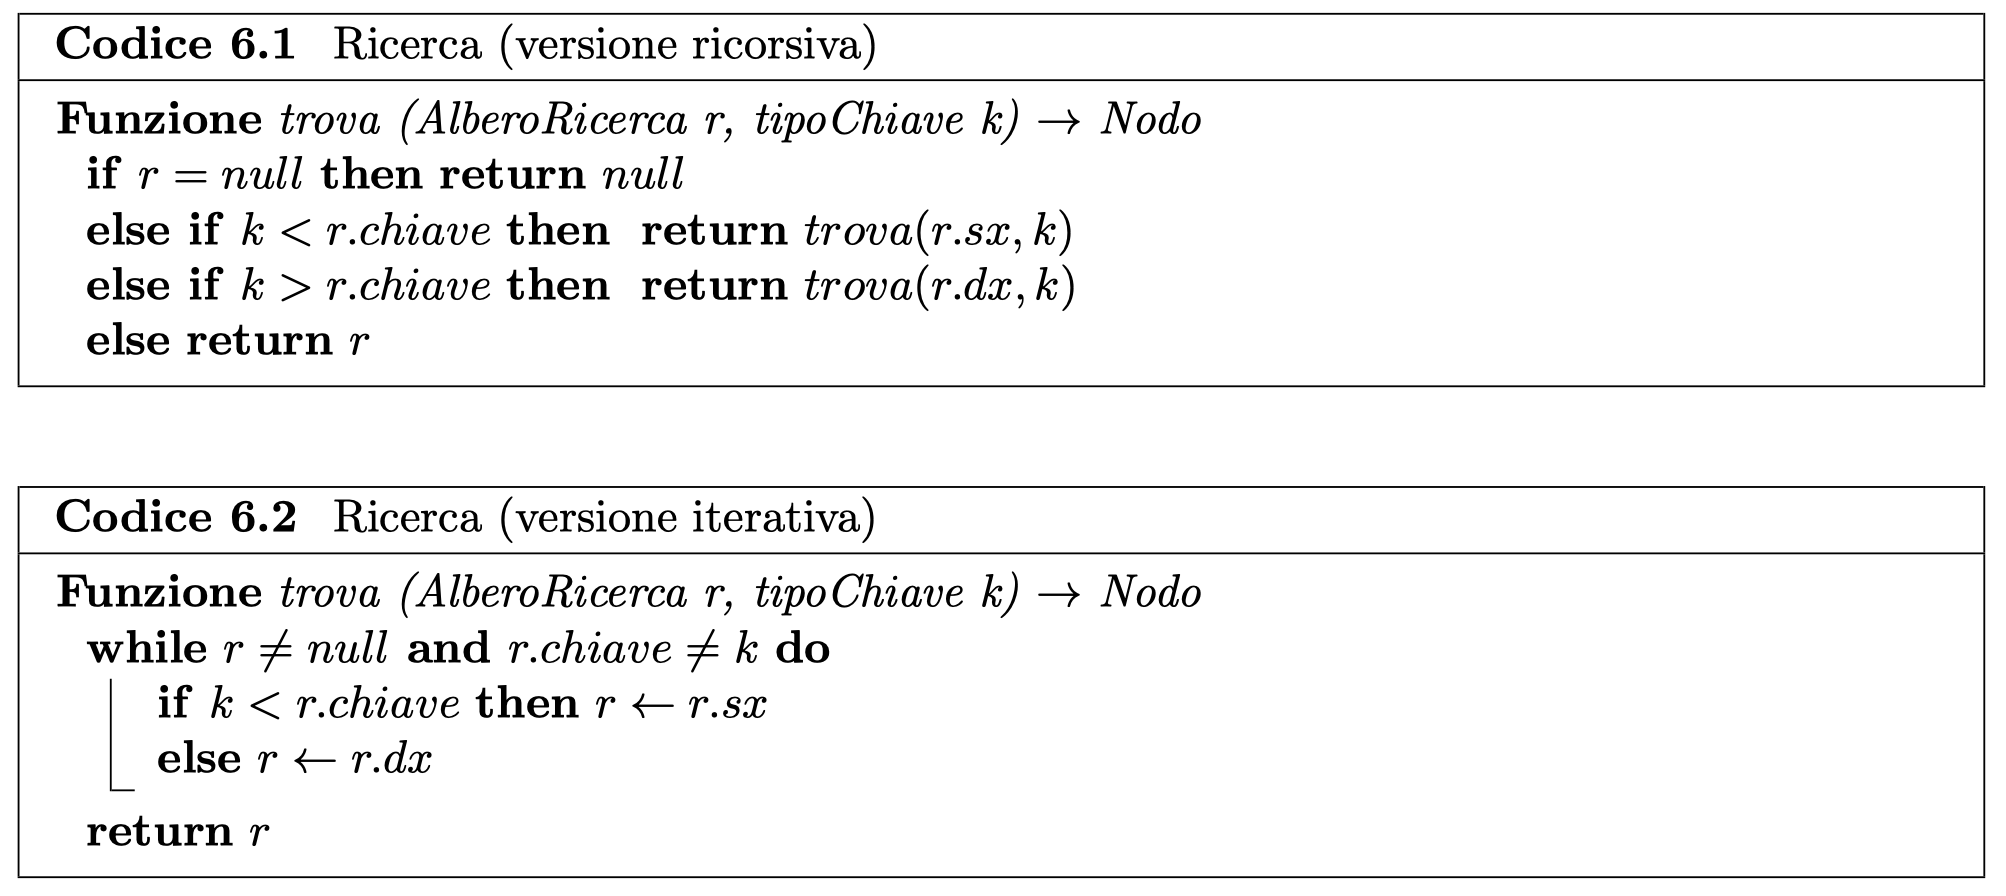
\includegraphics[width=\textwidth]{ricerca_abr.png}
\end{figure}

\begin{figure}[h]
    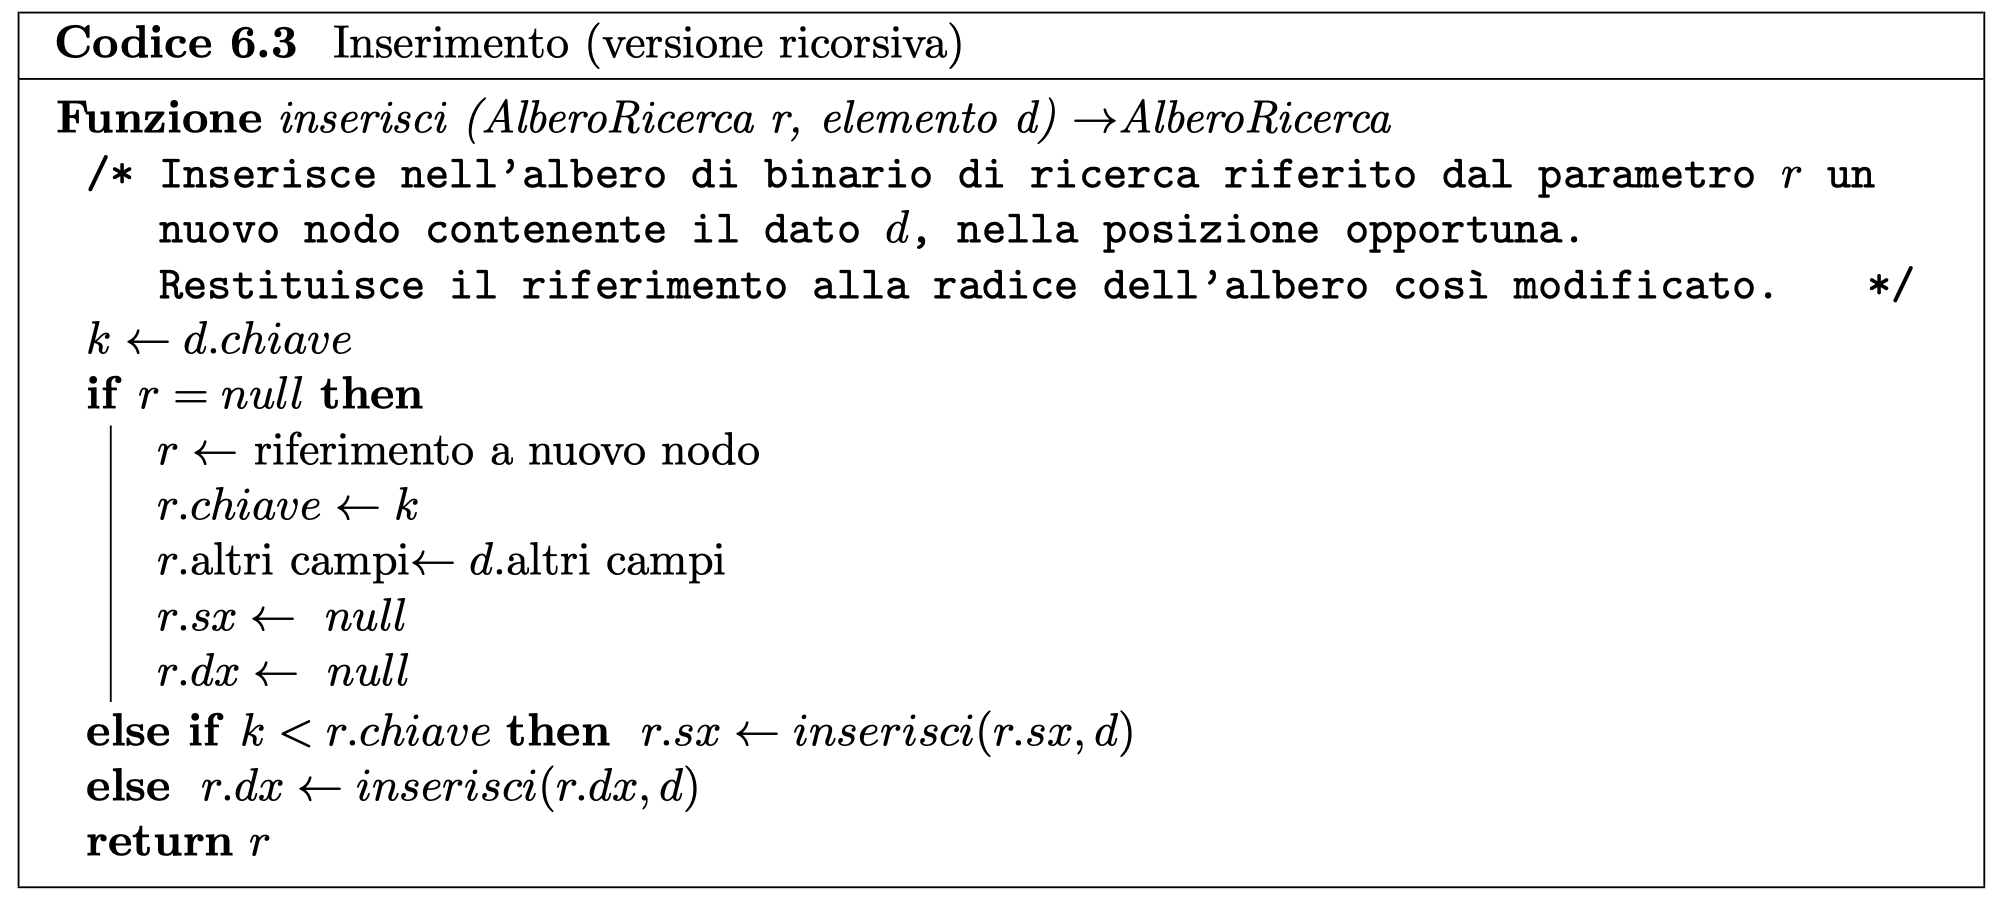
\includegraphics[width=\textwidth]{inserimento_ricorsivo_abr.png}
\end{figure}

\begin{figure}[h]
    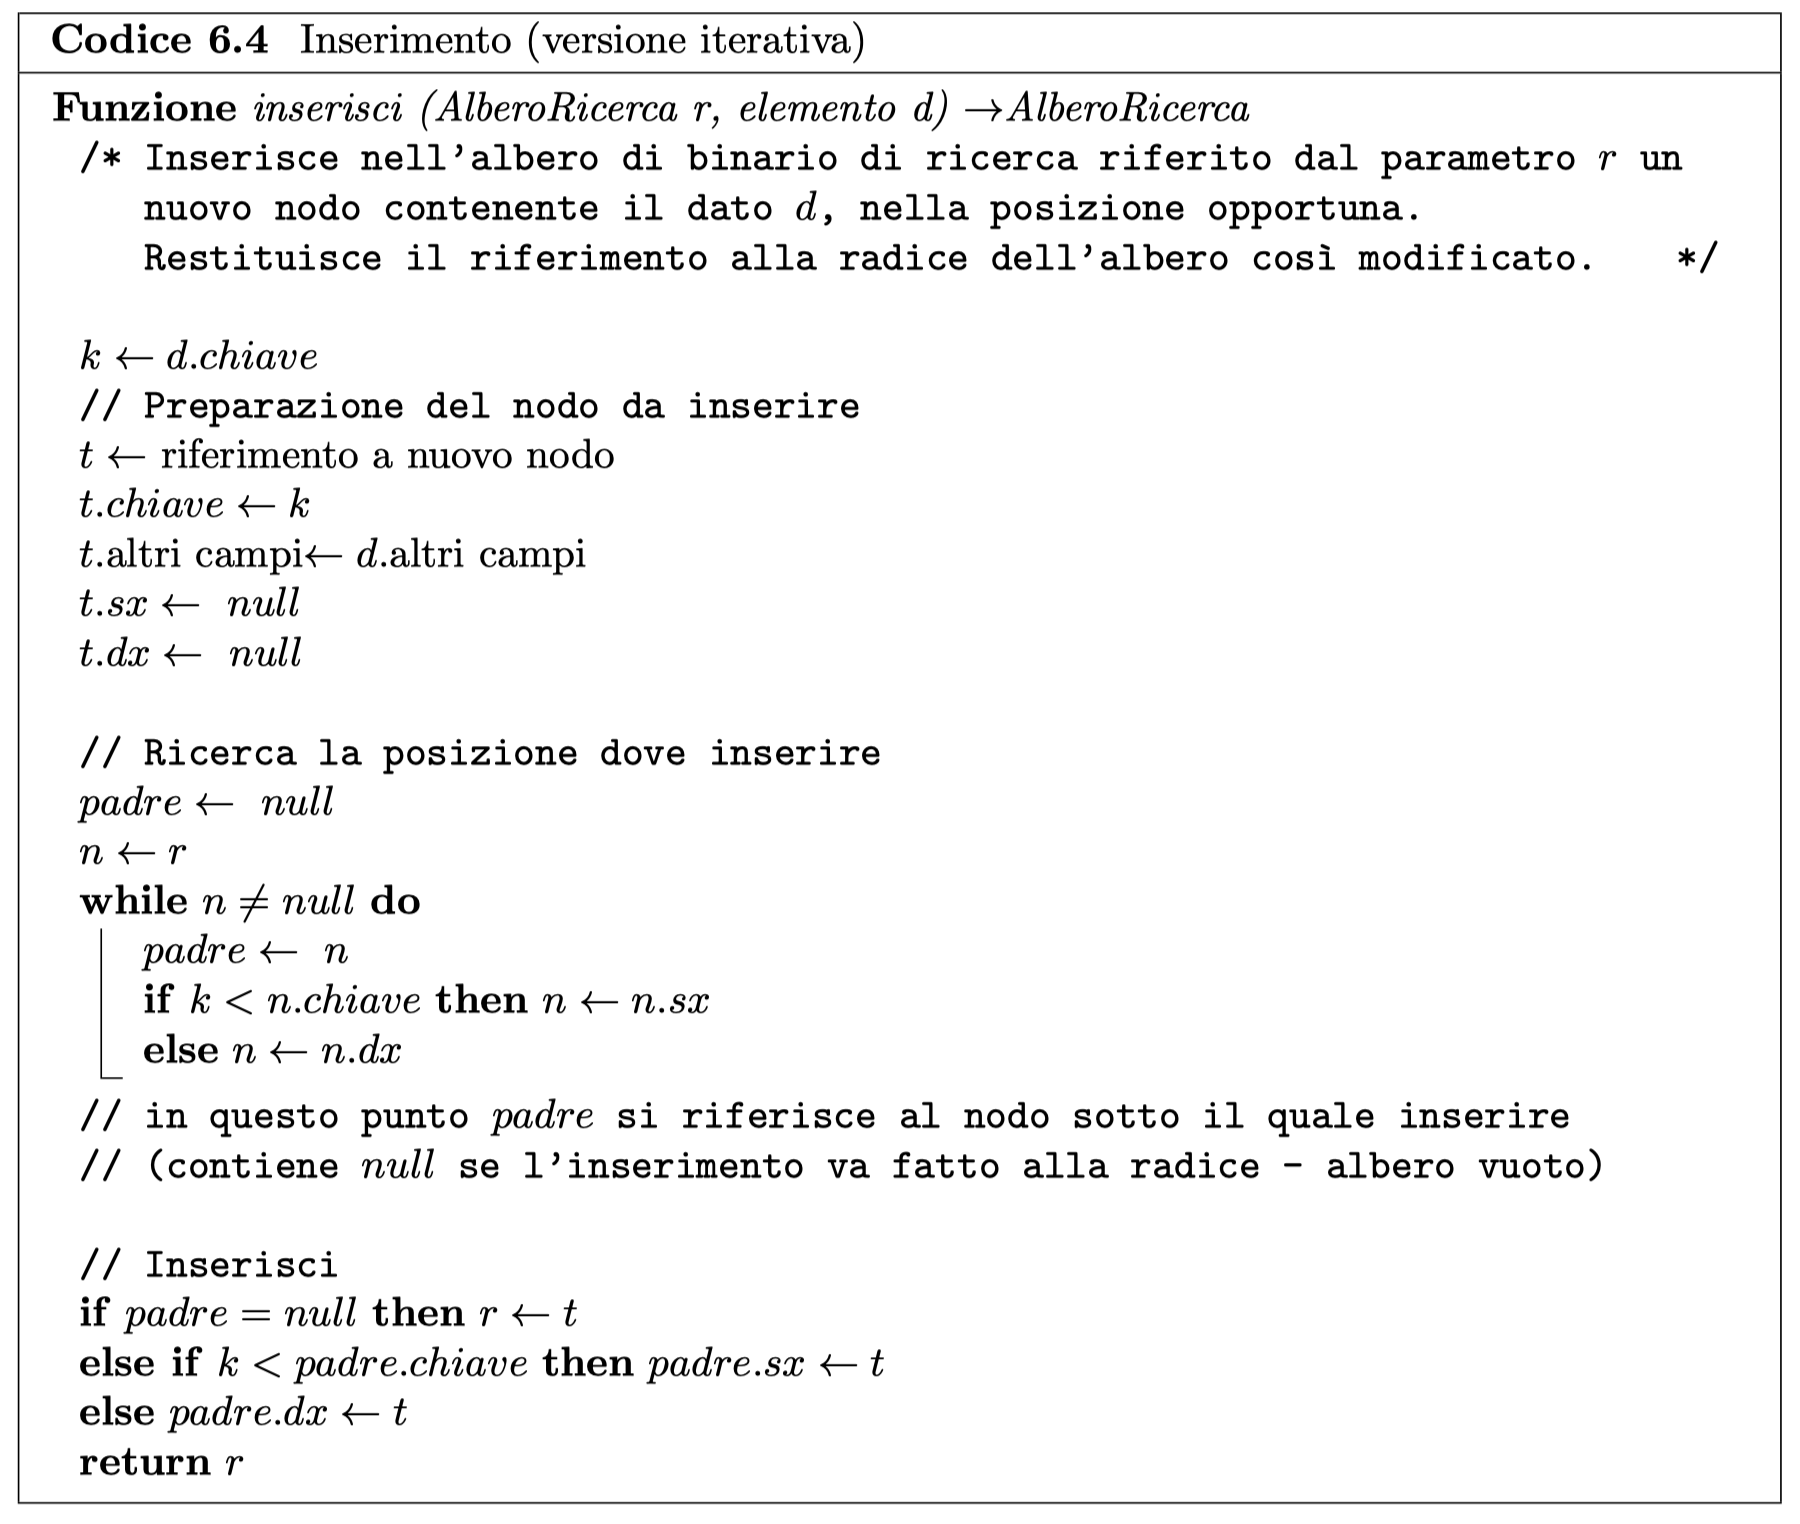
\includegraphics[width=\textwidth]{inserimento_iterativo_abr.png}
\end{figure}

\begin{figure}[h]
    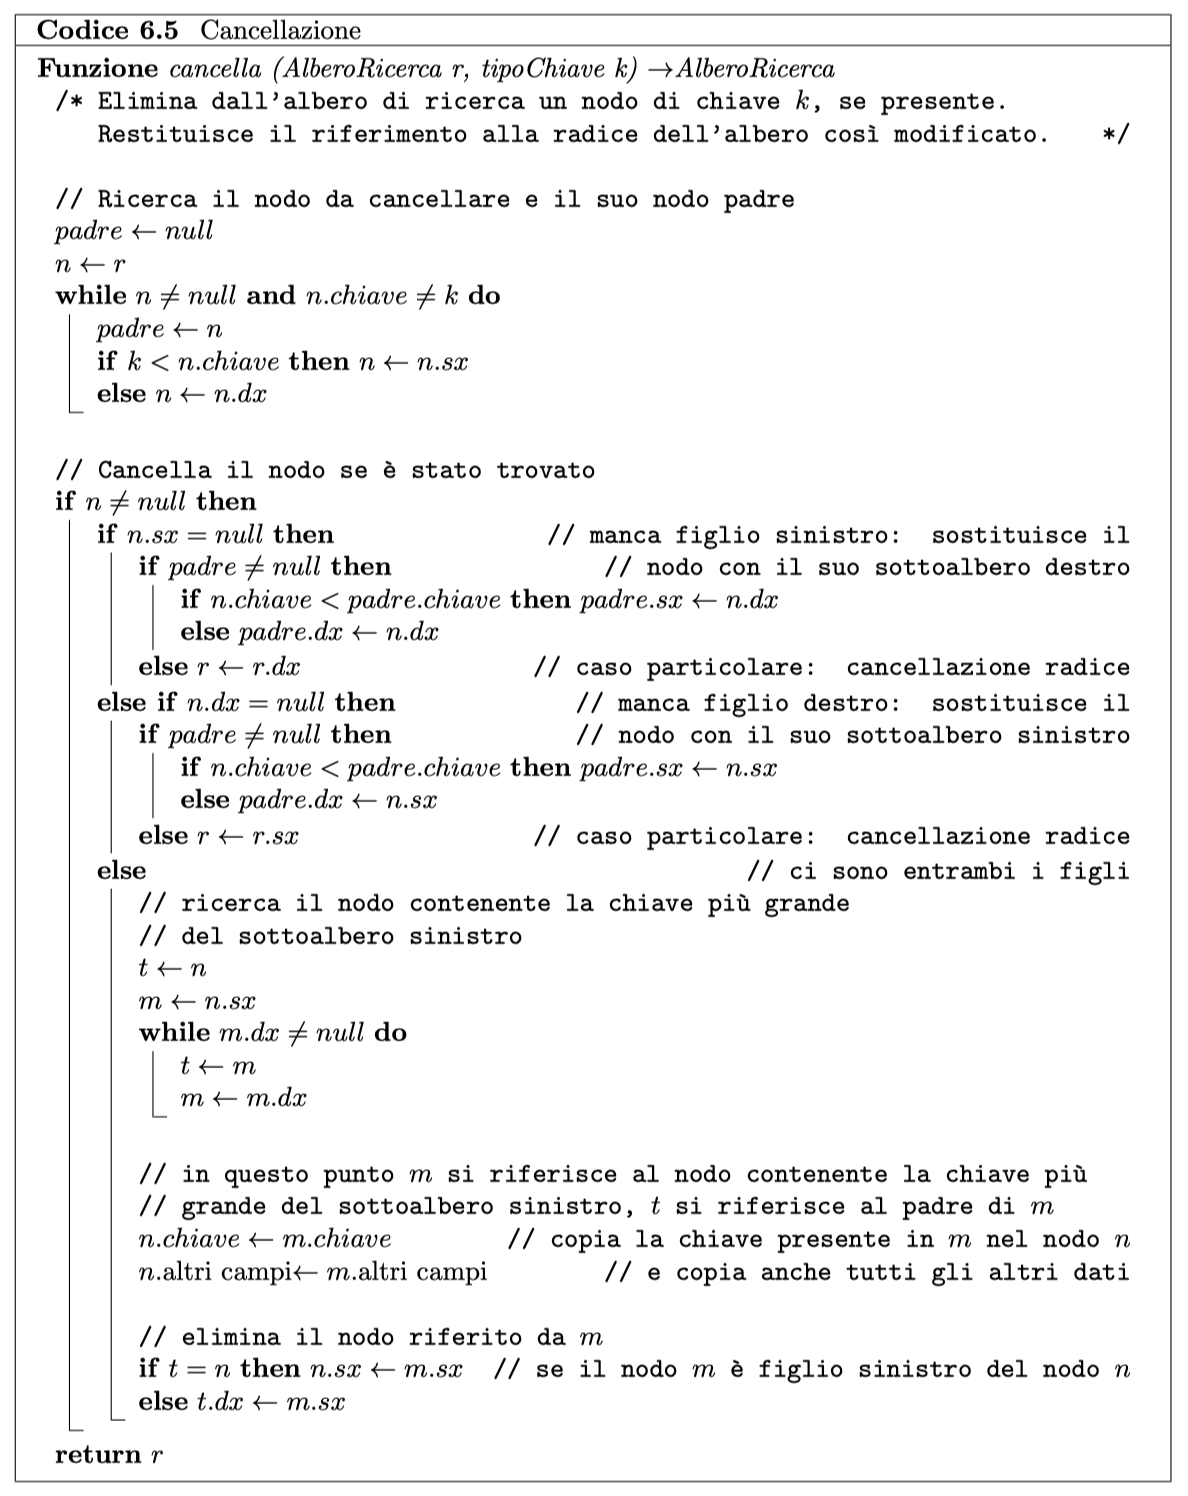
\includegraphics[width=\textwidth]{cancellazione_abr.png}
\end{figure}
\clearpage
